\chapter{Совместное использование сильно и слабо размеченных набооров данных} \label{chapt3}

\section{Мотивация} \label{sect3_1}

Как было сказано в предыдущей главе, классический MIL имеет ряд ограничний в том числе на размер карты. Поэтому были сформулированы следущие задачи:

\begin{itemize}
    \item Создать систему, которая способна возвращать карты сегментации высокого разрешения;
    \item Оснастить данную систему возможностью обучаться как на сильно так и на слабо размеченных наборах данных;
\end{itemize}

При решении даннных задач было обращено внимание на \cite{retinopathy}, где авторы уже решали подобную задачу. Они предложили пирамидальную интегральную структуру слоёв нейросети, которая один за одним последовательно суммирует с различными коэффициентами значения слоёв сети, с каждым шагом увеличивая размерность. В результате ряда экспериментов, мы остановились на архитектуре, изображенной на рис. \ref{fig:schema_total}. При этом предлагается следующий порядок обучения системы(рис. \ref{fig:schema_order}):

\begin{figure}[h] 
  \center
  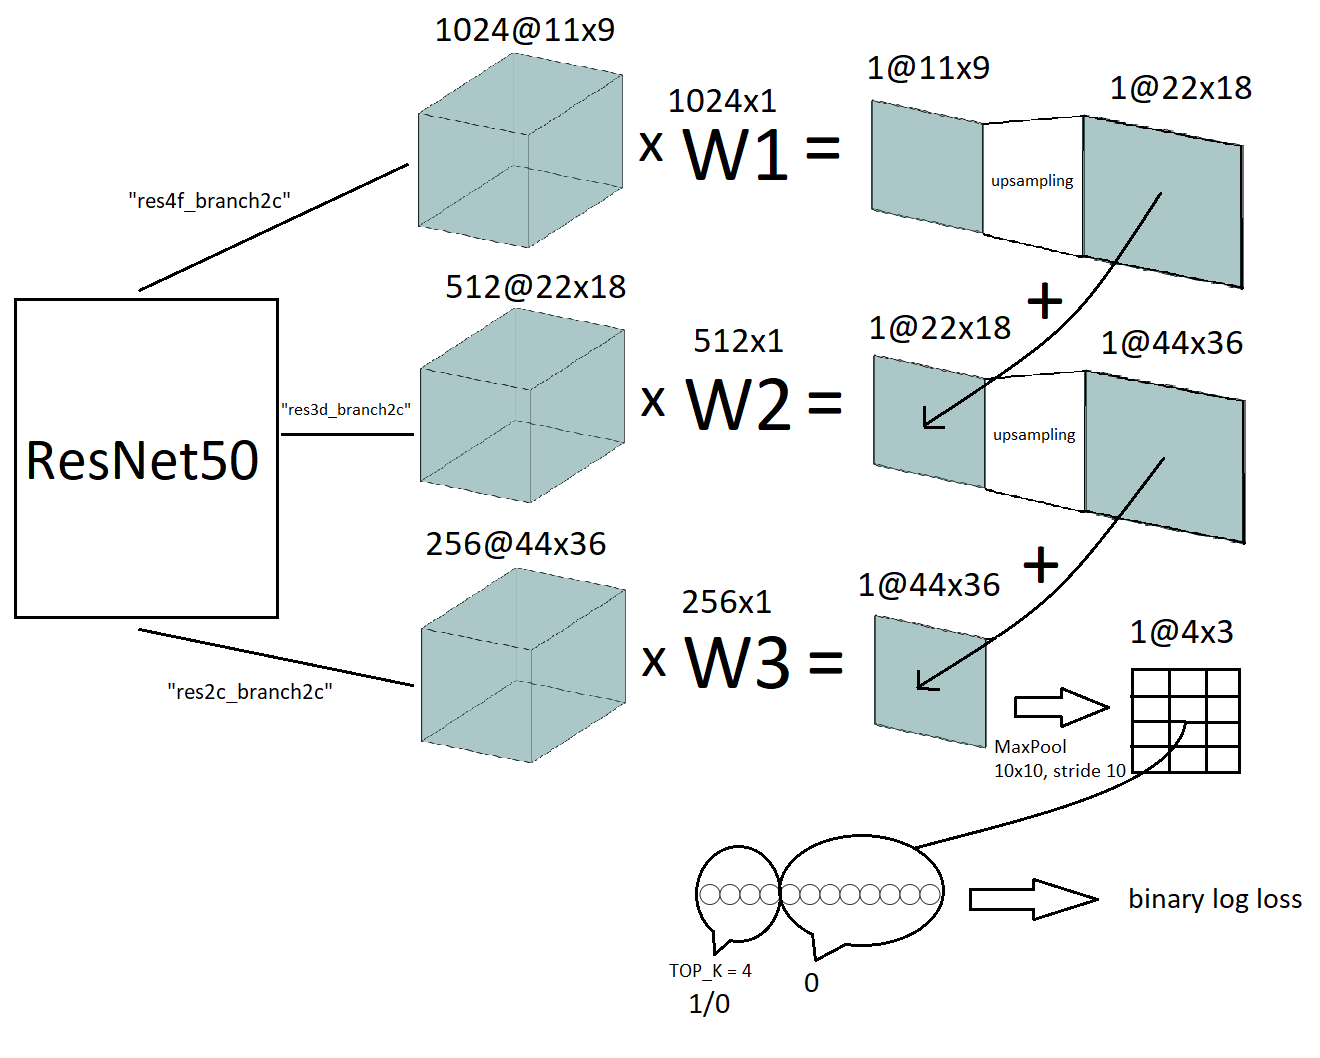
\includegraphics [scale=0.64] {images/schema_total.png}
  \caption{Схема архитектуры} 
  \label{fig:schema_total}  
\end{figure}


\begin{figure}[h] 
  \center
  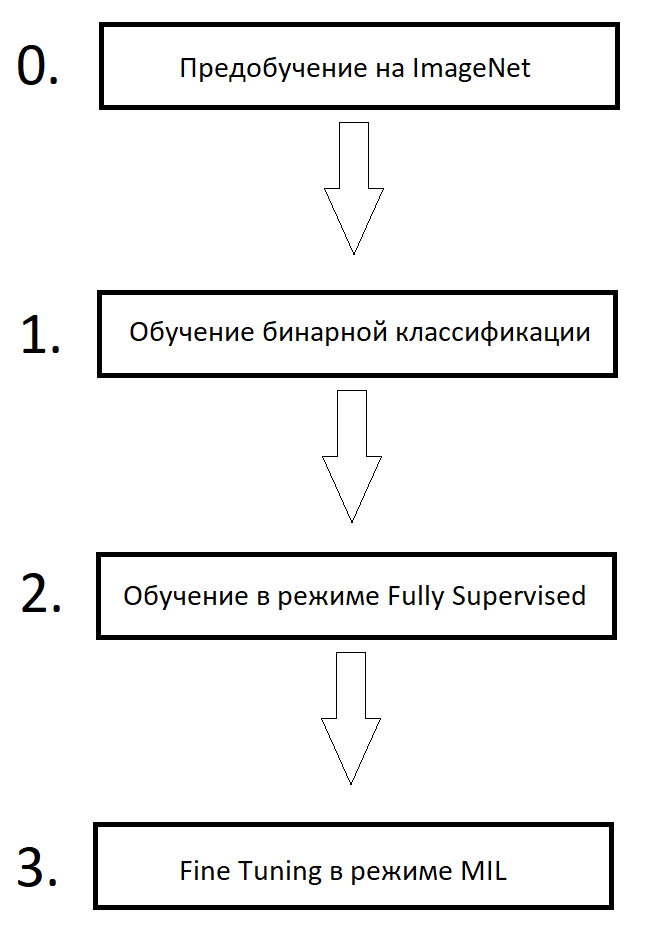
\includegraphics [scale=0.6] {images/schema.png}
  \caption{Порядок обучения} 
  \label{fig:schema_order}  
\end{figure}


\begin{enumerate}[start=0]
    \item Инициализация весов ResNet-50 весами после предобучения на ImageNet позволяет ускорить дообучение геометрических признаков, так как часть геометрических конфигураций уже усвоена сетью;
    \item Данный пункт будет изучен ниже. Выдвигается гипотеза, что, поскольку, распределение данных на ImageNet сильно отличается от распределения медицинских изображений, то имеет смысл сперва обучить классификацию, чтоб сеть <<адаптировала>> извлекаемые признаки под новое распределение, а затем переходить к обучению сегментации;  
    \item Далее идёт обучение сегментации на карте 44x36 с использованием сильной разметки на сильно размеченном наборе данных(малая часть данных);
    \item После этого предлагается улучшить полученную сегментацию путём применения метода MIL;
\end{enumerate}
На рис.\ref{fig:arch_class} изображена использованная архитектура модели классификации. Модели для всех трёх описанных видов обучения построены на основе {\bf одной и той же} модели ResNet-50 и имеют {\bf общие} слои с разделяемыми коэффициентами.

\begin{figure}[h] 
  \center
  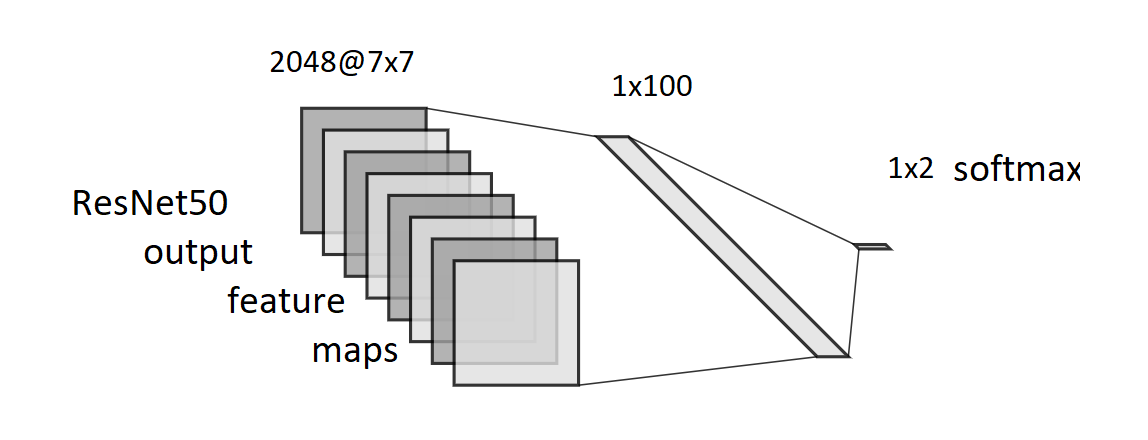
\includegraphics [scale=0.6] {images/arch_class.png}
  \caption{Архитектура модели классификации} 
  \label{fig:arch_class}  
\end{figure}



В последующих разделах будет обсуждаться подбор параметров системы и параметров обучения, предложенный порядок обучения(рис.\ref{fig:schema_order}), в частности, порядок следования пп.3 и 4, а также будут приведены численные результаты экспериментов с учётом кросс-валидации.

\section{Данные}

Для разработки системы сегментации нами были использованы данные конкурса по сегментации новообразований в мозге BRATS2018. Данный набор данных содержит 285 пациентов с диагнозом глиома. Для каждого пациента предоставлен набор слоёв МРТ в аксиальной проекции. Для каждого слоя дана попиксельная разметка опухоли, если она представлена в данном сечении. Сегментированная опухоль также разделена на несколько составных частей, однако мы в своей работе используем сегментацию опухоли целиком("whole tumor" на изображении ниже \ref{fig:bratss}).  Томографические снимки могут исполняться в различных контрастах. В наших экспериментах был использован контраст T1Gd. 

\begin{figure}[ht] 
  \center
  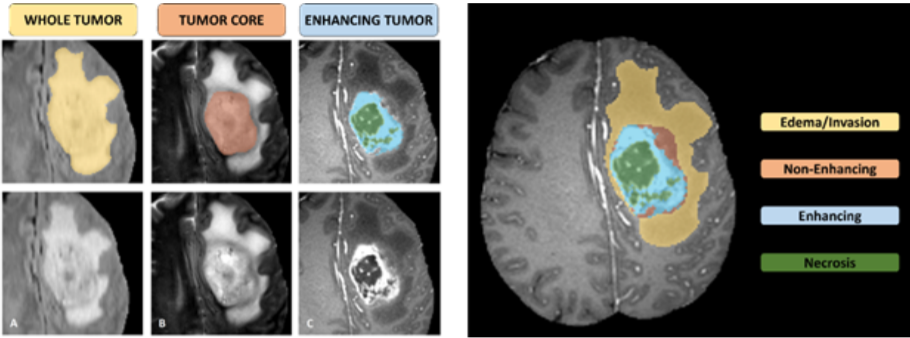
\includegraphics [scale=0.6] {images/brats.png}
  \caption{ Пример изображения мозга с сегментацией новообразования и его составных частей} 
  \label{fig:bratss}  
\end{figure}
Поскольку проекции мозга имеют различную площадь, крайние сечения могут быть существенно малы в сравнении с центральными сечениями. По этой причине крайние сечения, имеющие зачастую отличающуюся от средних сечений форму, были выброшены из рассмотрения. Всего число отобранных снимков варьируется от 98 до 123 и в среднем составляет {\bf 110}. Соотношение числа снимков, содержащих опухоль, к снимкам, ее не содержащим, варьируется от 0.22 до 9.18 и в среднем составляет {\bf 1.25}. Общее число изображений составляет {\bf 31350}, в т.ч. 15761 снимков, содержащих опухоль. 

Для каждого пациента серия снимков была выровнена таким образом, чтоб минимизировать фоновую площадь изображения(см. \ref{fig:transform}). Затем все изображения были приведены к формату 170x140.

\begin{figure}[ht] 
  \center
  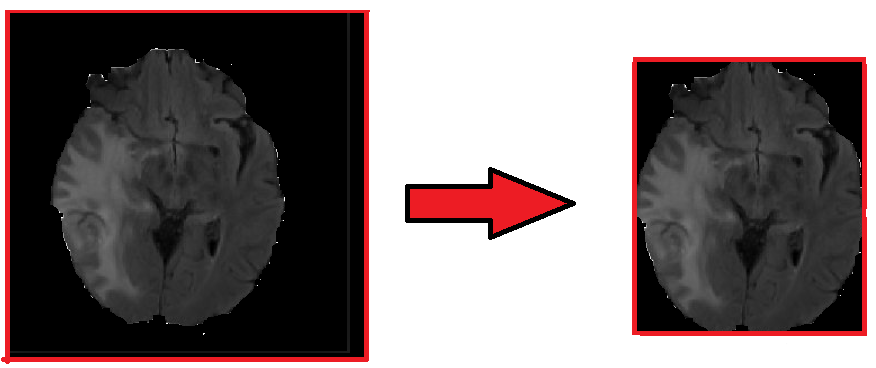
\includegraphics [scale=0.6] {images/transform.png}
  \caption{ Пример выравнивания серии изображений по крайним для нее достижимым границам изображения} 
  \label{fig:transform}  
\end{figure}

С целью упрощения реализации задач данной ранной работы на даннном этапе при выборе слоёв, содержащих опухоль, мы ограничились случаями, в которых опухоль занимает не менее 10\%, 5\% и 1\% от площади сечения {\bf мозга}(без фона) на изображении. Таким образом, были получены три набора данных:

\begin{center}
\begin{tabular}{||c |c ||} 
 \hline
  & Число изображений,  \\ [0.5ex]
  Выборка & содержащих опухоль \\
 \hline\hline
 \ge 10\% & 5636  \\ 
 \hline
 \ge 5\% & 9804 \\
 \hline
 \ge 1\% & 13806  \\[1ex] 
 \hline

 \hline
\end{tabular}
\end{center}
Впоследствии будет произведён анализ работы алгоритма на каждом из этих наборов данных.


\section{Метрика}

Прежде всего, следует определиться насчёт метрики для обучения на сильно размеченном наборе данных(fully supervised learning - будем обозначать {\bf FS}- обучение). 

Для задачи сегментации при обучении на данных с попиксельной разметкой обычно используют два вида метрик:
\begin{itemize}
    \item Индекс сходства Дайса(Dice index);
    \item Перекрестная энтропия(Binary crossentropy);
\end{itemize}

$$\text{Dice~index}(P,T) := \frac{2\sum_{i,j}P_{ij}T_{ij}}{\sum_{i,j}P^2_{i,j} + \sum_{i,j}T^2_{i,j}},$$
где P-пиксельная карта - предсказание($P_{i,j}\in [0,1]$), T - бинарная пиксельная карта($T_{i,j}\in\{0,1\}$). В качестве функции потерь при постановке задачи оптимизации метрики в терминах минимизации используют функцию потерь Дайса(Dice loss):

$$\text{Dice~loss} := 1 - \text{Dice~index}$$

Во избежание возможных проблем с делением на ноль используют параметр сглаживания(smooth), который часто берут равным 1:

$$\text{Dice~index}(P,T) := \frac{2\sum_{i,j}P_{ij}T_{ij} + smooth}{\sum_{i,j}P^2_{i,j} + \sum_{i,j}T^2_{i,j} + smooth},$$

Функция перекрёстной энтропии определяется следующим образом:

$$\text{Binary~crossentropy}(P, T) := -\sum_{i,j}\Large[T_{i,j}\log{P_{i,j}} + (1-T_{i,j})\log{(1-P_{i,j})}\Large]$$

В дальнейшем обе эти метрики будут использованы и сравнены друг с другом с точки зрения результатов эксперимента. Поскольку индекс Дайса имеет понятную геометрическую интерпретацию(отношение пересечения множеств к сумме их размеров), будем опираться на этот параметр при интерспретации результатов.

\section{Постановка эксперимента}

Сперва зададимся значением параметра $K = 4$. Будем варьировать следущие факторы:

\begin{itemize}
    \item Функция потерь, на которой происходит обучение в режиме FS: функция потерь Дайса или перекрёстная энтропия;
    \item Размер сильно размеченной выборки. Будем варьировать его следующим образом: 100, 300, 500, 1000, 2000; 
\end{itemize}

\subsubsection{Технические детали}

Эмпирическим путём был установлен следующий порядок обучения.

\begin{enumerate}

	\item Предобучение на массивном наборе данных ImageNet; в данной работе использована нейросеть ResNet-50 с уже предобученными на ImageNet весами,
	так что данный этап упоминается чисто формально;

	\item Обучение {\bf бинарной классификации}; обучение происходит в режиме Early Stopping 3 epochs(останавливаем процесс обучения, когда 
	нет улучшений потерь на валидационном наборе данных в течение 3 подряд идущих эпох) с сохранением и последующей подгрузкой лучших полученных за время обучения весов;
	
	\item Обучение сегментации fully supervised ({\bf FS}) на относительно небольшом наборе данных с сильной разметкой в режиме Early Stopping 5 epochs(аналогично предыдущему, только для 5 подряд идущих 
	эпох обучения);
	
	\item Обучение метода MIL(будем также говорить - fine tuning модели - {\bf FT}) производилось в режиме Early Stopping 1 epoch с толерантностью к улучшению Dice loss, равной 0.01(все меньшие улучшения таковыми не считались);
	
	\item При обучении тренировочная и валидационная выборки балансировались по числу изображений положительного и отрицательного класса(сперва выбиралось возможное число положительных с учётом выборки(1\%, 5\% или 10\%), затем бралось такое же число изображений, не содержащих опухоли)

\end{enumerate}

При оптимизации использовался метод оптимизации Adam. При этом шаг оптимизации(learning rate) для классификации и FS-обучения выбирался равным $5*10^{-5}$, а для FT-обучения снижался пропорционально размеру сильно размеченного набора данных(эвристика).


\subsection{Результаты эксперимента}

Как было упомянуто выше, необходимо понять, какуя функция потерь лучше всего использовать для FS-обучения. 

В таблицах ниже приведены результаты эксперимента. Читать таблицы следует следущим образом:

\begin{itemize}
    \item По строкам - результаты для этапов 5-перекрёстной оптимизации;
    \item <<LR>> - шаг обучения;
    \item <<Classifier Acc>> - точность предобученной бинарной классификации;
    \item <<Dice Loss Val FS>> - Dice loss для  FS-обучения, полученный при валидационной выборке - в случае прямого обучения FS на Dice loss и в случае непрямого(LogLoss) соответственно;
    \item <<Dice Loss Val FT>> -  полученный на валидационной выборке итоговый Dice loss для FT-обучения(MIL) над результатом FS-обучения - в случае прямого обучения FS на Dice loss и в случае непрямого(LogLoss) соответственно;
    \item Строка <<AVG>> - среднее по столбцам c доверительными интервалами Стьюдента по пяти значениям кросс-валидации;
    \item Данные в каждой таблице для разделов <<Dice>> и <<Logloss>> посчитаны на одном и том же для данной таблицы разбиении, а значит, позволяют сравнивать эти два подхода.
\end{itemize}

\begin{figure}[ht] 
  \center
  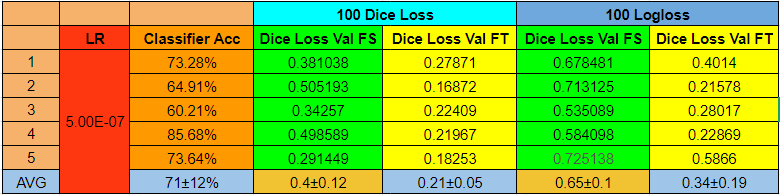
\includegraphics [scale=1.0] {images/experiment_100.png}
  \caption{ Результаты для эксперимента с 50 сильно размеченными изображениями для FS (+50 не содержащих опухоли- итого 100) } 
\end{figure}

\begin{figure}[ht] 
  \center
  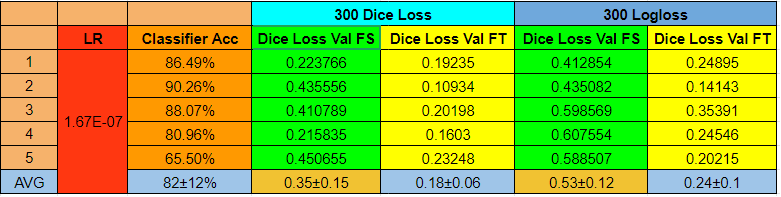
\includegraphics [scale=1.0] {images/experiment_300.png}
  \caption{  Результаты для эксперимента со 150 сильно размеченными изображениями для FS (+150 не содержащих опухоли- итого 300) } 
\end{figure}

\begin{figure}[ht] 
  \center
  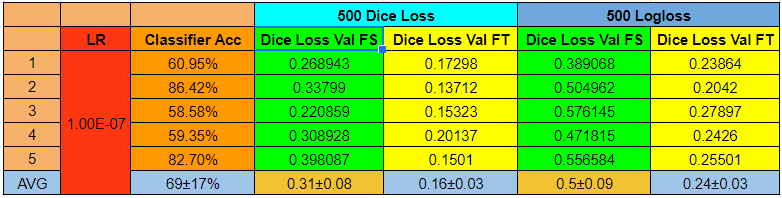
\includegraphics [scale=1.0] {images/experiment_500.png}
  \caption{  Результаты для эксперимента со 250 сильно размеченными изображениями для FS (+250 не содержащих опухоли- итого 500)} 
\end{figure}

\begin{figure}[ht] 
  \center
  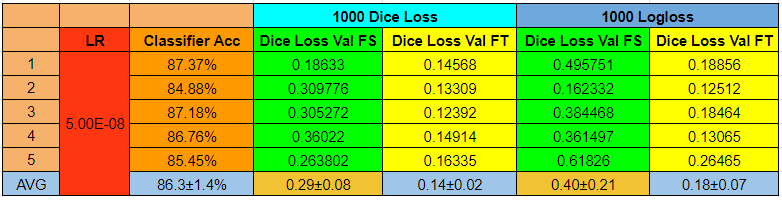
\includegraphics [scale=1.0] {images/experiment_1000.png}
  \caption{  Результаты для эксперимента с 500 сильно размеченными изображениями для FS (+500 не содержащих опухоли- итого 1000)} 
\end{figure}

\begin{figure}[ht] 
  \center
  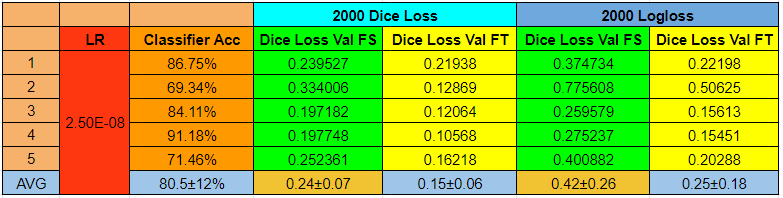
\includegraphics [scale=1.0] {images/experiment_2000.png}
  \caption{  Результаты для эксперимента с 1000 сильно размеченными изображениями для FS (+1000 не содержащих опухоли- итого 2000)} 
\end{figure}

Также дополним полученные таблицы графиком, в котором <<dice-fs>>, <dice-ft>>, <log-fs>>, <log-ft>> соответствуют упомянутым в пояснениях к таблицам выше категориям. 

\begin{figure}[ht] 
  \center
  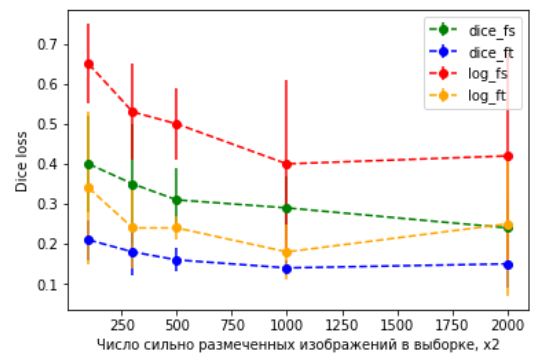
\includegraphics [scale=1.0] {images/plot_results.png}
  \caption{ Результаты эксперимента} 
\end{figure}

{\bf Вывод:} из графиков видно, что подход с прямой оптимизацией на FS более выгоден с точки зрения итогового индекса Дайса после FT- обучения.
\section{Необходимость классификаци}

С тем чтобы установить необходимость предобучения на бинарной классификации, был поставлен следующий эксперимент: для одного и того же разбиения(5-кросс-валидации) было произведено FS - обучение в двух случая:
\begin{itemize}
    \item С предварительным предобучением на задаче бинарной классификации;
    \item Без предварительного предобучения на задаче бинарной классификации;
\end{itemize}

Из результатов, отражённых в таблице, следует, что нельзя говорить об положительном эффекте предобучения. Статистически получается то же самое среднее значение.


\begin{figure}[ht] 
  \center
  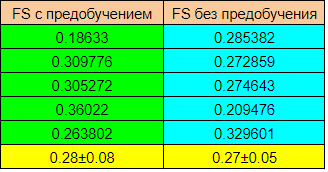
\includegraphics [scale=1.0] {images/cmp_pretrain.png}
  \caption{ Сравнение результатов с предобучением и без} 
\end{figure}


\section{Подбор значения параметра К}

Данный параметр будем подбирать в отдельности для каждого из выбранных наборов данных. 


\clearpage